\documentclass{article}

\usepackage{listings}
\usepackage{color}
\usepackage{graphicx}
\usepackage{float}
\usepackage{amsmath}
\usepackage{subfig}
\usepackage{cite}
\usepackage{url}
\usepackage{amsmath}

\newcounter{qcounter}

\begin{document}

\title{Image Analysis - TP4 - K Means}

\author{Jander Nascimento, 
\and Raquel Oliveira}

\maketitle

\section{Initial concept}

The \emph{k-means} split the image in \emph{k} sets based in some parameters. Those parameters are heuristics to split the set. One common way to split the sets is in a 3d space, in which the domain of the space is [0,255] and each axle is the color space RGB. 

The algorithm is composed of the following steps:
\begin{list}{\arabic{qcounter}:~}{\usecounter{qcounter}}
\item Given a number of regions \emph{k}, randomly generate the initial values of the means $m_1, m_2, ..., m_k$, which are called \emph{centroids}.
\item Assign each pixel to the group that has the closest centroid.
\item When all pixels have been assigned, recalculate the $m_k$ values of the \emph{k} centroids.
\item Repeat Steps 2 and 3 until the centroids no longer move. This produces a separation of the pixels into groups.
\end{list}

\begin{figure}[H]
\centering
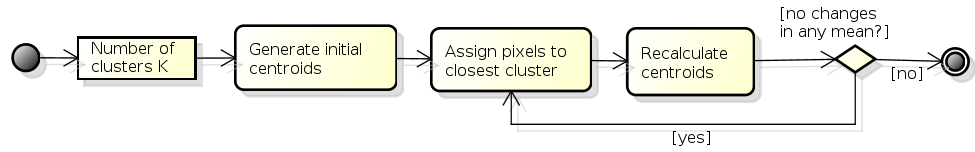
\includegraphics[width=1.0\textwidth]{../image/ActivityDiagram.png}
\caption{K-means steps}
\label{fig:kmeans}
\end{figure}

\section{Initial \emph{k} influences}

The results produced depend on the initial values for the means (centroids). The simplest way is to select these values randomly, although the better choice is to place them far away as much as possible from each other.


\section{Number of regions}

\emph{K} represents the number of clusters that is going to be used in the segmentation process. 
This information is fundamental to distinguish the number of regions in the image, so as bigger \emph{k} is, more cluster are going to be used, therefore more detailed the image will be.  

In the current implementation we used the color intensity as the orthogonal space, with the axis(x,y,z) been represented by the color red, green and blue of the pixel.

The difference can be seen in the Figure \ref{fig:clusters}. The \ref{fig:k2} use only two distinct groups, so the image presents two segments, which does not give too many details about the image.  In the \ref{fig:k3} with three groups, is possible to see more details than in the previous image. In \ref{fig:k10} we can see that the details in the image increases dramatically.

\begin{figure}[H]
	\centering
	\subfloat[Original Image]{\label{fig:original}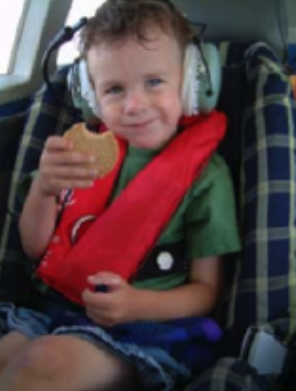
\includegraphics[width=0.3\textwidth]{image/image2}}
	\hspace{0.1cm}
	\subfloat[K=2]{\label{fig:k2}
\includegraphics[width=0.3\textwidth]{image/image2-2}}
	\hspace{0.1cm}
	\subfloat[K=3]{\label{fig:k3}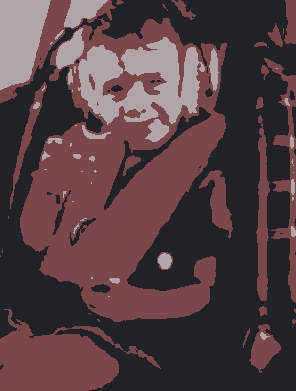
\includegraphics[width=0.3\textwidth]{image/image2-3}}
	\hspace{0.1cm}
	\subfloat[K=10]{\label{fig:k10}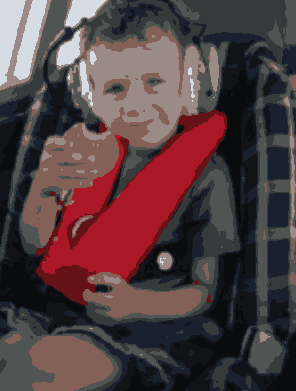
\includegraphics[width=0.3\textwidth]{image/image2-10}}
	\hspace{0.1cm}
	\caption{K-Means}
	\label{fig:clusters}
\end{figure}

\section{Other influences}

\subsection{Including distance between pixels}

Using the distance as a factor to determine the groups allows not only create groups based in the color space distance, but also based in the distance between the group and the pixel. 

In the Figure \ref{fig:distance} it was used the same number of clusters (\emph{k}) for the tested image.

It is clear that using the distance as an information, the edges of the objects are better defined. If we do not consider the distance some objects are simply merged based in how close the colors are from each other, which is not always the case. As shown in the Figure \ref{fig:nodist} the objects were almost completely merged because of the proximity to the green color.

\begin{figure}[H]
	\centering
	\subfloat[Original Image]{\label{fig:distori}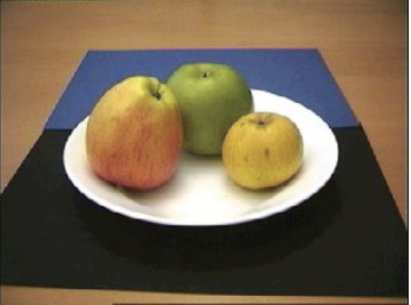
\includegraphics[width=0.3\textwidth]{../image/Q4-original}}
	\hspace{0.1cm}
	\subfloat[Not considering distance]{\label{fig:nodist}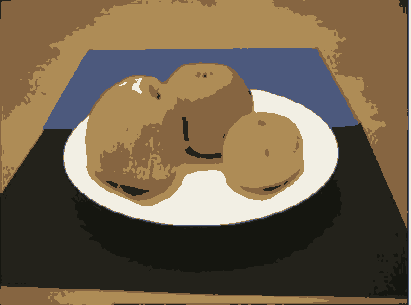
\includegraphics[width=0.3\textwidth]{../image/Q4-nodistance}}
	\hspace{0.1cm}
	\subfloat[Considering distance]{\label{fig:dist}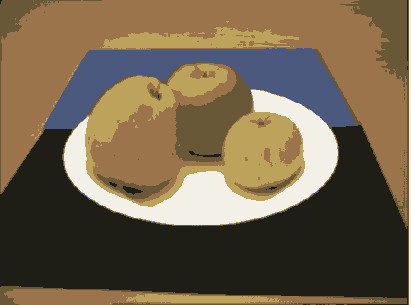
\includegraphics[width=0.3\textwidth]{../image/Q4}}
	\caption{Using distance between pixels as an information}
	\label{fig:distance}
\end{figure}

This result can be achieved simply by adding the Euclidean distance for the distance between the pixels. The Equation \ref{equa:diff} should be applied to the intensities red, green and blue and the Euclidean distance between the pixel position.
\begin{equation}
 \operatorname{arg\,min}\sum_{i=1}^{K}\sum_{x_j \in S_i}^{} \|x_j-\mu_i\|
\label{equa:diff}
\end{equation}

\subsection{Balancing distance and colors influence}

Since the influence of the distance, as the color, are not the same for every image, is possible to increase or decrease its influence by using a contribution factor, so this adjustment can be done independently.

	\subsection{How to run?}

	Steps to compile the application:
	
	\begin{itemize}
		\item svn checkout https://jfimageanalysis.googlecode.com/svn/trunk/TP4/ \#download source code
		\item make \#compiles the code
	\end{itemize}

	As an input image only {\bf ppm plaintext/ansii} files are accepted (P3). 

	Examples of usage:

	\begin{itemize}
		\item Create 3 clusters:
		\subitem ./showregion -i image\_in.pgm -g 3 $>$ image\_out.pgm
	\end{itemize}

	You can always type {\it ./imagetransform --help} to check for more options. 

\end{document}


